\documentclass{beamer}
\mode<presentation>
{
  \usetheme{Berkeley}
  \usecolortheme{dolphin}
  \useinnertheme{rounded}
}

\usepackage[slantfont,boldfont]{xeCJK}
\setmainfont{Times New Roman}
\setCJKmainfont{Songti SC}
 \setCJKfamilyfont{song}{Songti SC}



%\setCJKmainfont{Songti SC}   % STFangsong 设置缺省中文字体
%\setCJKmonofont{STFangsong}   % 设置等宽字体
%\setCJKsansfont{Songti SC}
%\setmainfont{Heiti TC} % 英文衬线字体
%\setmonofont{STFangsong} % 英文等宽字体
%\setsansfont{Times} % 英文无衬线字体

\usepackage{tikz}%绘图
\usetikzlibrary{positioning} %on grid
\usetikzlibrary{automata} %style
\usepackage{fontspec}%字间距控制?
\usepackage{tikz}%绘图
\usetikzlibrary{positioning} %on grid
\usetikzlibrary{automata} %style?
\usetikzlibrary{shapes,snakes}%各中形状
%%%%%%%%%%%%%%%%%%%
\usepackage[english]{babel}
% or whatever


\usepackage{caption}

\usepackage{times}
\logo{
\includegraphics[height=0.1\textwidth]{figures/tjdx.png}}

\title[图灵奖获得者介绍] % (optional, use only with long paper titles)
{1976年图灵奖获得者}
\subtitle
{Michael O. Rabin,  Dana Steward Scott}

\author[ly \and syh]% (optional, use only with lots of authors)
{林胤\and 孙渊汇}

\institute
{
  同济大学电子与信息学院
}



\AtBeginSection[]
{
  \begin{frame}<beamer>{内容提纲}
    \tableofcontents[currentsection,currentsubsection]
 \end{frame}
}
\begin{document}


\begin{frame}
  \titlepage %封面
\end{frame}
\begin{frame}{内容提纲}
  \tableofcontents
\end{frame}

\section{生平简介}
\begin{frame}{1976年的两位图灵奖得主}
\pause
\begin{figure}[htbp]
	\begin{minipage}{0.4\textwidth}
	\centering
		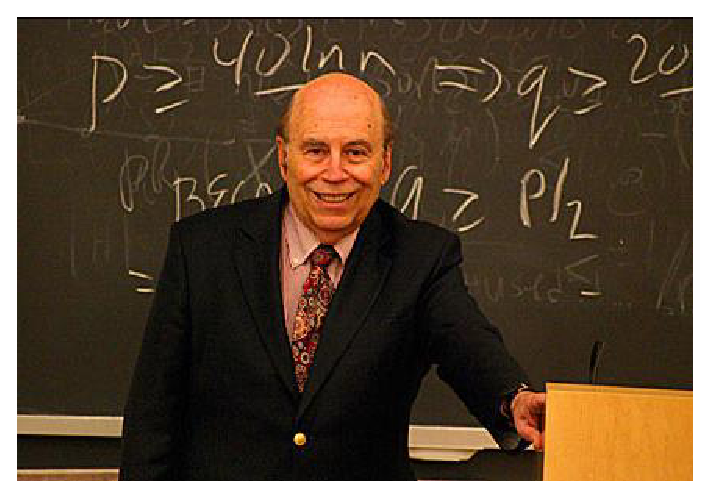
\includegraphics[scale=0.3]{figures/lb2.eps}
		\caption*{Michael O. Rabin}
	\end{minipage}
	\pause
	\begin{minipage}{0.4\textwidth}
	\centering
		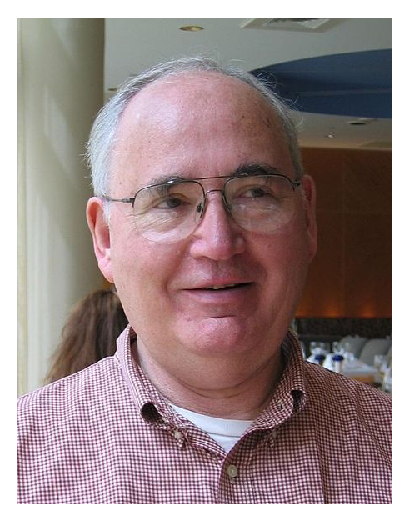
\includegraphics[scale=0.3]{figures/sct.eps}
		\caption*{Dana Steward Scott}
	\end{minipage}
\end{figure}
\end{frame}

\begin{frame}
  \begin{theorem}
    $A = B$.
  \end{theorem}
  \begin{proof}
    \begin{itemize}
    \item Clearly, $A = C$.\pause
    \item As shown earlier,  $C = B$.\pause
    \item Thus $A = B$.\pause
    \end{itemize}
  \end{proof}
  \begin{example}
  here is example
  \end{example}
\end{frame}

\section{图灵和可计算性}
\section{能够进行猜想的计算机}
\section{计算的固有难度}
\section{抛硬币做决定的计算机}

\end{document}

